\chapter{Impementace do systému Kelvin}
\label{ch:implementation}

Předchozí kapitola~\ref{ch:selection} popsala výběr modelu, způsobu nasazení a promptovací strategie pro integraci LLM do systému Kelvin.
Tato kapitola se věnuje samotné realizaci navrženého řešení: konkrétnímu způsobu začlenění LLM modulu do architektury systému, průběhu komunikace s jazykovým modelem, prezentaci výsledků učiteli v uživatelském rozhraní a evaluačnímu nástroji využitému pro ověření kvality jednotlivých konfigurací.

% =============================================================
\section{Backend}
\label{sec:implementation-backend}

Implementace LLM modulu na straně backendu byla realizována jako samostatná část Django aplikace (modul), která rozšiřuje systém Kelvin o nový asynchronní krok navazující vedle existující synchronní evaluaci odevzdání.
Tato sekce popisuje integraci do evaluační pipeline, strukturu modulu, průběh asynchronní analýzy, konfiguraci jazykových modelů a způsob ukládání výsledků.

\subsection{Integrace do evaluačního procesu}
\label{subsec:implementation-pipeline}

Při odevzdání řešení studentem systém Kelvin spustí evaluační proces zajišťující kompilaci, automatické testy a provedení učitelem vytvořené pipeline.
Souběžně je spuštěn modul LLM analýzy, který ke své práci potřebuje výhradně zdrojové soubory studenta, dostupné ihned po odevzdání.
Paralelní běh je možný proto, že výsledky evaluace nejsou pro LLM analýzu vyžadovány, a zároveň přirozený — výstupy analýzy jsou určeny pouze učiteli a student na ně nečeká, podobně jako u asynchronní kontroly plagiátorství.

Začlenění výsledků evaluace do vstupu LLM analýzy by naopak vyžadovalo sekvenční zpracování a prodloužilo dobu čekání.
Otevřelo by však prostor pro propracovanější analýzu: model by mohl pracovat i s výstupy kompilátoru, například s varováními nebo chybami nástroje Clang, a ve svých návrzích na ně přímo odkazovat.
Toto rozšíření tak představuje přirozený směr dalšího rozvoje implementace.

\begin{figure}[h]
    \centering
    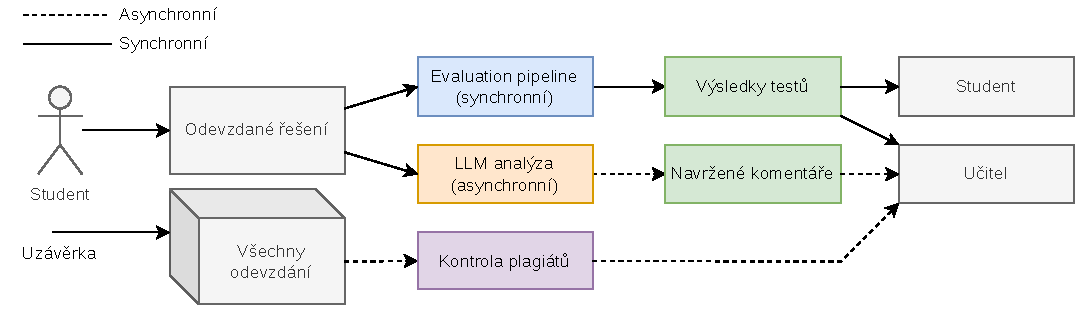
\includegraphics[width=1.0\textwidth]{resources/diagrams/evaluation-pipeline}
    \caption{Zjednodušené schéma zpracování odevzdání v systému Kelvin, znázorňující paralelní běh synchronní evaluační pipeline a asynchronní LLM analýzy}
    \label{fig:implementation-pipeline}
\end{figure}

\endinput
\subsection{Struktura modulu}
\label{subsec:implementation-module}

LLM modul je uspořádán jako standardní Django aplikace složená z osmi hlavních souborů a několika souborů v~API vrstvě, přičemž každý z nich pokrývá jasně ohraničenou část funkcionality.
Toto rozdělení odděluje logiku komunikace s jazykovým modelem od správy promptů, definice výstupního schématu a ukládání výsledků do databáze.
Výsledná adresářová struktura modulu je uvedena ve \lstref[výpisu]{lst:implementation-structure}.

\begin{listing}[H]
    \inputminted{awk}{resources/sources/file-structure.txt}
    \caption{Struktura adresářů a souborů implementace}
    \label{lst:implementation-structure}
\end{listing}

\endinput
\subsection{Asynchronní úloha a průběh analýzy}
\label{subsec:implementation-job}

Samotný průběh analýzy je řízen asynchronní úlohou definovanou v souboru \texttt{job.py}, která je při zpracování odevzdání volána souběžně se spuštěním evaluační pipeline.
Úloha je zcela nezávislá na synchronní části evaluace a prochází několika na sebe navazujícími kroky.

Nejprve jsou pomocí funkcí z modulu \texttt{processor.py} shromážděny všechny zdrojové soubory patřící k~danému odevzdání.
Každý soubor je převeden na objekt \texttt{EmbeddedFile}, který obsahuje relativní cestu v~rámci odevzdání, identifikovaný programovací jazyk, úplný obsah souboru a celkový počet řádků.
Tento formát umožňuje modelu pracovat s~plným kontextem souboru a současně mu poskytuje strukturovaná metadata.

Následně je z databáze načten prompt definovaný pro danou úlohu v~její konfiguraci.
Prompty jsou uloženy jako samostatné záznamy a lze je upravovat prostřednictvím administračního rozhraní systému Kelvin, aniž by bylo nutné nasazovat novou verzi aplikace (viz \secref{subsec:implementation-prompts}).
Konkrétní režim analýzy je rovněž načten z konfigurace a může nabývat hodnot \texttt{CHAIN\_OF\_THOUGHT}, \texttt{ZERO\_SHOT} nebo \texttt{THINKING} (viz \secref{subsec:prompts-strategies}).

Poté je vytvořena instance třídy \texttt{Analyzer} s klientem knihovny \texttt{openai} poskytnutým modulem \texttt{openai\_config.py}.
Třída \texttt{Analyzer} obdrží seznam souborů, prompt a zvolený režim a provede samotnou komunikaci s~jazykovým modelem.
Po dokončení komunikace je odpověď modelu zpracována pomocnými funkcemi z modulu \texttt{processor.py}, které ji parsují do seznamu objektů \texttt{SuggestedCommentDTO} a uloží je do databáze jako instance Django modelu \texttt{SuggestedComment}.

V případě selhání kteréhokoli kroku, například nedostupnosti LLM serveru, chyby při parsování odpovědi nebo překročení časového limitu, je úloha označena jako neúspěšná a do databáze se nic neukládá.
Informace o selhání je zaznamenána do logu systému a zároveň je administrátorům odeslána notifikace formou emailu, což umožňuje rychlou reakci a řešení problému.

\endinput
\subsection{Konfigurace jazykových modelů}
\label{subsec:implementation-config}

Modul podporuje připojení k více OpenAI-kompatibilním serverům prostřednictvím konfiguračního souboru \code{openai-config.yaml}.
Každý záznam v tomto souboru definuje adresu serveru, autentizační token, popis serveru, možné modely a zda je tento server výchozí pro zpracování odevzdání.
Při inicializaci modulu je ověřeno, zda konfigurační soubor existuje a pokud ne, je vytvořen s výchozí konfigurací obsahující jediný záznam pro lokální server Ollama\@.

Výchozím serverem je lokálně provozovaná instance Ollama, která umožňuje spouštět jazykové modely přímo na infrastruktuře školy.
Toto nastavení bylo zvoleno s ohledem na dvě hlavní omezení popsaná v sekci \secref{sec:llm-limitations}: finanční náklady spojené s využíváním cloudových API a částečná ztráta kontroly nad daty při odesílání studentských kódů do externích služeb.

V případě potřeby lze konfiguraci rozšířit o cloudové poskytovatele, například OpenAI nebo jiné OpenAI-kompatibilní alternativy, aniž by bylo nutné měnit kód aplikace.

\endinput
\subsection{Třída Analyzer a režimy analýzy}
\label{subsec:implementation-analyzer}

Komunikace s jazykovým modelem je zapouzdřena ve třídě \texttt{Analyzer} v souboru \texttt{llm\_reviewer.py}.
Třída přijímá seznam objektů \texttt{EmbeddedFile} připravených v souboru \texttt{job.py}, nakonfigurovaného klienta knihovny \texttt{openai} a zvolený režim analýzy.
Knihovna \texttt{openai} poskytuje jednotné rozhraní pro všechny OpenAI-kompatibilní servery, takže stejný kód funguje jak pro lokální instanci Ollama, tak pro cloudové poskytovatele.

Centrálním vstupním bodem třídy je metoda \texttt{process}, která na základě zvoleného režimu orchestruje celý průběh analýzy.
Při volbě režimu \texttt{ZERO\_SHOT} nebo \texttt{THINKING} je provedeno jediné volání příslušné analytické metody.
Při volbě \texttt{CHAIN\_OF\_THOUGHT} jsou postupně spuštěny tři fáze -- \textbf{hrubá analýza}, \textbf{kritická revize} a \textbf{finální shrnutí} -- přičemž výstup každé fáze je předán jako kontext fázi následující.
Srovnání režimů z pohledu kvality výstupů a doby zpracování je uvedeno v \secref[sekci]{subsec:choice-strategies}.

\subsubsection*{Normalizace názvu souboru}
\label{subsubsec:implementation-analyzer-normalization}

Po dokončení analýzy je výsledek předán metodě \texttt{normalize\_issue\_filenames}.
Jazykové modely v názvech souborů občas vynechávají část cesty nebo ji mírně pozměňují.
Metoda proto každý vrácený název porovná se skutečnými vstupními cestami pomocí postupné shody přípon, prefixů a základního názvu a při jednoznačné shodě název opraví.
Tím je zajištěno, že každý nalezený problém odkazuje na platný soubor bez ohledu na to, jak jeho cestu model zapsal.

Toto opatření reaguje na konkrétní případy zjištěné během testování.
Studenti občas odevzdají soubor, ke kterému operační systém při duplicitních názvech připojí číselnou příponu (např.\ \texttt{main.c~(1)}).
Některé modely tuto příponu ve svém výstupu vynechávají, což následně vede k chybám při mapování problému na správný soubor.
V jiných případech modely nahrazují původní název generickým; například soubor \texttt{MIK0486.c} byl ve výstupu některých modelů uveden pouze jako \texttt{main.c}.

\endinput
\subsection{Zpracování výstupu a datový model}
\label{subsec:implementation-model}
 
Odpověď jazykového modelu je zpracována pomocnými funkcemi v souboru \code{processor.py}, které parsují strukturovaný výstup modelu do seznamu objektů \code{SuggestedCommentDTO}.
Každý objekt obsahuje cestu k souboru, číslo řádku, textový obsah návrhu a závažnost nálezu.
 
Výsledné objekty jsou ukládány do databáze jako instance Django modelu \code{SuggestedComment}.
Model je propojen s odpovídajícím odevzdáním (\code{Submit}) a obsahuje následující klíčová pole.
 
\begin{itemize}
    \item \code{source} obsahuje cestu k analyzovanému souboru v rámci odevzdání.
    \item \code{line} uchovává číslo řádku, ke kterému se návrh vztahuje.
    \item \code{text} obsahuje vlastní obsah návrhu vygenerovaný modelem.
    \item \code{severity} vyjadřuje závažnost nálezu a nabývá hodnot \code{CRITICAL}, \code{HIGH}, \code{MEDIUM} nebo \code{LOW}.
    Tato hodnota slouží k vizuálnímu rozlišení návrhů ve frontendu.
    \item \code{state} uchovává aktuální stav návrhu a nabývá hodnot \code{PENDING}, \code{ACCEPTED}, \code{REJECTED} nebo \code{DISMISSED}.
    \item \code{quality\_rating} a \code{relevance\_rating} obsahují hodnocení kvality a relevance na stupnici 0 až 10, pokud jej učitel udělil.
\end{itemize}
 
Datový model je využíván pro dva typy záznamů.
Prvním typem jsou jednotlivé návrhy komentářů vázané na konkrétní řádek zdrojového kódu, u kterých učitel volí mezi stavy \code{ACCEPTED} a \code{REJECTED}.
Druhým typem je celkové informativní shrnutí odevzdání, které nelze přijmout, protože má pouze informativní charakter.
U shrnutí může učitel využít výhradně stav \code{DISMISSED}, kterým jej ve svém rozhraní skryje.
 
Pokud učitel jednotlivý návrh přijme, systém automaticky vytvoří standardní komentář v databázi, který je propojen s původním navrhovaným komentářem a stane se viditelným pro studenta.
Zamítnuté nebo skryté záznamy zůstávají v databázi pro účely pozdější analýzy kvality modelu a případné doladění promptů, ale studentovi nejsou zpřístupněny.
 
\endinput

% =============================================================
\section{Frontend}
\label{sec:implementation-frontend}

% =============================================================
\section{Nástroj pro analýzu kvality promptů}
\label{sec:implementation-tool}

\endinput